\documentclass[11pt]{article}

\usepackage[margin=1in]{geometry}
\usepackage[T1]{fontenc}
\usepackage{lmodern}
\usepackage{microtype}
\usepackage{amsmath}
\usepackage{amssymb}
\usepackage{graphicx}
\usepackage{array}
\usepackage{booktabs}
\usepackage{float}
\usepackage{caption}
\usepackage{tikz}
\usetikzlibrary{arrows.meta,positioning,fit,calc,decorations.pathmorphing}
\usepackage{hyperref}

\hypersetup{
  colorlinks=true,
  linkcolor=blue,
  urlcolor=blue,
  pdftitle={Simulating RREA with Feedback in an RZ Particle-in-Cell Code},
  pdfauthor={RREA WarpX/AMReX project},
  pdfkeywords={RREA, relativistic feedback, TGF, WarpX, AMReX,
    particle-in-cell, photometer}
}

\setlength{\parindent}{0pt}
\setlength{\parskip}{0.7em}
\renewcommand{\arraystretch}{1.18}
\emergencystretch=1.5em

% Shared colour grammar with the architecture guide: orange = our code,
% blue = stock WarpX, green = the native library / fluid family.
\colorlet{rreafill}{orange!12}
\colorlet{rreaedge}{orange!60!black}
\colorlet{warpxfill}{blue!8}
\colorlet{warpxedge}{blue!50!black}
\colorlet{nativefill}{green!10}
\colorlet{nativeedge}{green!45!black}

\title{Simulating RREA with Feedback in an RZ Particle-in-Cell Code}
\author{RREA WarpX/AMReX project}
\date{}

\begin{document}
\maketitle

\begin{abstract}
\noindent
This note describes a hybrid kinetic/fluid particle-in-cell model of
relativistic runaway electron avalanches in a realistic thundercloud field, and
the pipeline that turns its output into the quantities instruments record.
Kinetic runaway electrons, positrons and photons are coupled to a low-energy
fluid whose conductivity discharges the field driving the avalanche, in
cylindrical symmetry, on the open-source WarpX and AMReX frameworks. The field
solve is Maxwell at finite propagation speed. Optical emission in the
photometer bands is driven by the native ion-pair source and transported to the
observer through the cloud. This note assumes RREA and relativistic feedback are
familiar and particle-in-cell methods are not; the architecture guide remains
the reference.
\end{abstract}

\section{What this code is}

A thundercloud region above the RREA threshold multiplies runaway electrons;
bremsstrahlung photons and pair-produced positrons can travel back upstream and
seed fresh avalanches; if each avalanche seeds on average more than one
successor, the process becomes self-sustaining. What such an event would look
like to an instrument --- in shape and timing; absolute amplitudes follow the
assumed seed --- is what this model exists to predict.

The model solves that whole system at once: everything in
Figure~\ref{fig:loop} is computed in one run, each element reacting to the
others every time step.

\begin{figure}[H]
  \centering
  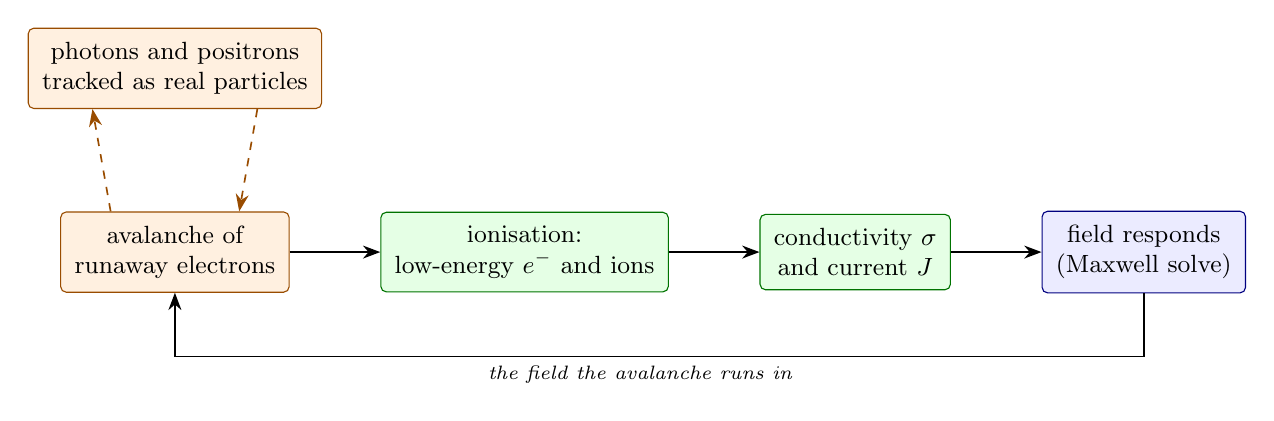
\begin{tikzpicture}[
      node distance=6mm,
      box/.style={draw, rounded corners=2pt, align=center, font=\small,
                  inner sep=5pt, minimum height=9mm},
      arr/.style={-{Stealth[length=2.2mm]}, semithick},
      fb/.style={-{Stealth[length=2.2mm]}, semithick, dashed, rreaedge}
    ]
    \node[box, fill=rreafill, draw=rreaedge] (aval)
      {avalanche of\\runaway electrons};
    \node[box, fill=nativefill, draw=nativeedge, right=11.5mm of aval] (ion)
      {ionisation:\\low-energy $e^-$ and ions};
    \node[box, fill=nativefill, draw=nativeedge, right=11.5mm of ion] (sigma)
      {conductivity $\sigma$\\and current $J$};
    \node[box, fill=warpxfill, draw=warpxedge, right=11.5mm of sigma] (field)
      {field responds\\(Maxwell solve)};

    \draw[arr] (aval) -- (ion);
    \draw[arr] (ion) -- (sigma);
    \draw[arr] (sigma) -- (field);
    \draw[arr] (field.south) -- ++(0,-8mm)
      -| node[pos=0.26, below, font=\scriptsize\itshape]
        {the field the avalanche runs in} (aval.south);

    \node[box, fill=rreafill, draw=rreaedge, above=13mm of aval] (carriers)
      {photons and positrons\\tracked as real particles};
    \draw[fb] ($(aval.north west)!0.22!(aval.north east)$)
      -- ($(carriers.south west)!0.22!(carriers.south east)$);
    \draw[fb] ($(carriers.south west)!0.78!(carriers.south east)$)
      -- ($(aval.north west)!0.78!(aval.north east)$);
  \end{tikzpicture}
  \caption{The loop that is closed here. Solid path: the avalanche creates a
  low-energy plasma, which conducts, which discharges the field, which changes
  the avalanche the field is driving. Dashed path (left arrow up, right arrow
  down): photons and positrons are produced by the avalanche and carried as
  kinetic species, so they can travel back upstream and seed new avalanches.}
  \label{fig:loop}
\end{figure}

In one sentence: \textbf{this is a hybrid kinetic/fluid, electromagnetic
particle-in-cell model in cylindrical symmetry}, built on the open-source
WarpX/AMReX stack, with Monte Carlo charged-particle and photon transport from
Geant4-anchored interaction tables.

\section{How you solve a physics problem with a PIC code}
\label{sec:pic}

The name is slightly misleading: ``particle-in-cell'' is less about particles
than about the \emph{marriage} of particles and a mesh.

PIC answers two separate impossibilities. Computing every pair interaction is
$N^2$ with $N$ astronomically large; but particles need not see each other
individually, only the \emph{field} they collectively produce, so a mesh is
introduced as the meeting place. And for TGF, flickering-gamma-ray-flash and
glow production $N$ is of order $10^{16}$ runaway electrons and upward, which
no machine can hold or push,
so a simulated particle is never one electron but a weighted sample
(Section~\ref{sec:macro}). The loop below addresses the first:

\begin{enumerate}\itemsep2pt
  \item \textbf{Deposit.} Each particle's charge and current are spread onto the
    nearby mesh points. The mesh now holds the charge density $\rho$ and the
    current density $J$.
  \item \textbf{Solve.} A field equation is solved \emph{on the mesh}: here,
    Maxwell's equations at finite propagation speed (Section~\ref{sec:hybrid}).
    This is the global calculation, and where the collective physics happens.
  \item \textbf{Gather.} The field is interpolated from the mesh back to each
    particle's position.
  \item \textbf{Push.} Each particle is advanced by the equation of motion under
    the field it just received.
  \item \textbf{React.} Particles undergo collisions, ionisation, scattering,
    creation and loss; for us, Monte Carlo transport in air.
\end{enumerate}

Repeat, one time step at a time. The cost is now roughly linear in particle
number plus one field solve, which is what makes the problem tractable at all.

The conceptual point is step 2 feeding step 3. Because the field is recomputed
from the particles every step, and the particles are then moved by that
recomputed field, \textbf{the problem is self-consistent by construction}. That
is the property the loop of Figure~\ref{fig:loop} rests on: it is not something
added on top of PIC, it is what PIC \emph{is}, and the work lies in getting all
the other physics (transport, ionisation, conductivity, feedback carriers) to
live inside the same loop.

Two constraints come with the method and set the run cost. The mesh must resolve
the structures of interest, since anything smaller is invisible to the field
solve; its scale must be compared with the characteristic avalanche length.
The outer time step
must likewise keep $c\Delta t$ below the mesh spacing, and quantitative claims
still require spatial and temporal convergence.
Section~\ref{sec:macro} returns to what that sampling choice costs.

What PIC is good at: self-consistent collective behaviour, and kinetic
populations far from thermal equilibrium, both essential here. What it is bad
at: representing enormous numbers of low-energy particles individually, and
resolving structure below the mesh scale. Both shape
Section~\ref{sec:hybrid}.

\section{AMReX and WarpX}

AMReX provides the mesh, its distribution across MPI ranks, and the array and
communication primitives used by the explicit Maxwell update.
WarpX is a PIC code built on AMReX, developed for laser-plasma and accelerator
modelling, which is why it may be unfamiliar in this field; it supplies the loop
of Section~\ref{sec:pic} and a well-tested cylindrical (RZ) mode. The RREA
physics (the Monte Carlo air interactions, the low-energy fluid, the field
solve, the atmosphere profile) is added through an overlay without modifying
either dependency's pinned source tree.

A word on why the field solve is ours rather than WarpX's own electromagnetic
solver, since that is the obvious question. WarpX's EM loop is bound to its own
particle push and current deposition, and this model deliberately replaces the
push: the runaway transport owns each particle's trajectory, so WarpX would
deposit a path nobody flew. Its RZ material (conductive-medium) update is also
absent, and conduction is precisely the physics here. What we need instead is
small: axisymmetry with poloidal currents leaves exactly three field
components, so the solver is a few hundred lines that read the same face
currents the fluid already builds.

\section{The macroparticle, and why the population must be managed}
\label{sec:macro}

A simulated ``particle'' is not one electron. It is a \emph{macroparticle}: a
sample of phase space carrying a weight, the number of physical particles it
represents. The production source is a continuous cosmic-ray (PARMA)
electron/positron column plus its initial stationary population; the schedule
assigns weights so the sampled macros represent the integrated physical
fluence.

This is Monte Carlo sampling, not a fudge factor: the macroparticle follows the
equations of a single real electron, and the weight enters only when quantities
are summed. Weighting is not a convenience either, it is the only reason the
problem is computable. Following $10^{16}$ runaway electrons individually is
beyond any foreseeable machine by many orders of magnitude: at a few tens of
bytes of state each they would occupy hundreds of petabytes before a single
step is taken.
Sampling the same population with a finite macroparticle ensemble, each becoming
much heavier as multiplication proceeds, is what brings it into reach. The
cost is statistical resolution, since with fewer, heavier macroparticles the
noise is larger. What weighting does to the physics is a genuine assumption and
worth stating as one: for quantities that are simply sums over the population
the estimator can be unbiased, and that is the limit of what is guaranteed.
Once the sampled population feeds the nonlinear charge--conductivity--field
loop, the average of a function is not the function of the average. Increasing
the macro count is expected to reduce sampling error, but sufficiency must be
established separately for each observable with population-resolution and
ensemble ladders.

The complication specific to an avalanche is that the population
\emph{multiplies}, so macroparticle count would grow until memory ran out. When
the population reaches its control band the code performs a
\textbf{charge-exact stochastic thinning}.  It adjusts weights along the null
space of the four-cell CIC deposit, eliminating particles while leaving every
deposited cell charge unchanged in that realization.  Each particle's expected
weight is preserved, so thinning costs particle/spectral statistics without
injecting charge noise into the Maxwell field.

\section{Why cylindrical (RZ), and what it costs}
\label{sec:rz}

The simulation runs in cylindrical coordinates $(r,z)$ with azimuthal symmetry:
every quantity is independent of azimuth. The mesh is therefore
two-dimensional, while the physics (volumes, densities, the field solve) stays
fully three-dimensional, since each cell is a ring of revolution.

What this buys is decisive. Resolving the same radial extent with a full
three-dimensional mesh adds the missing azimuthal cells and makes kinetic
transport impractical. RZ replaces those cells by physically weighted rings,
making the production calculation tractable.

What it forbids is real: no azimuthal structure, no tilted or off-axis geometry,
no filamentary channels that break symmetry. The model describes an axisymmetric
avalanche column.

Axisymmetry also makes the exact axis a radiation null, which is why the
on-axis diagnostic of Section~\ref{sec:radio} is a longitudinal field, not
radio.

\section{The hybrid: kinetic runaways, fluid low-energy plasma}
\label{sec:hybrid}

Section~\ref{sec:pic} noted that PIC is bad at carrying enormous numbers of
low-energy particles. An RREA produces many more low-energy carriers than
runaways. Representing those
as macroparticles would swamp the run, and would be wasteful, because they
matter almost entirely through the \emph{conductivity} they provide.

So the model splits the plasma:

\begin{center}
\begin{tabular}{@{}>{\raggedright\arraybackslash}p{0.30\textwidth}>{\raggedright\arraybackslash}p{0.63\textwidth}@{}}
\toprule
\textbf{Kinetic species} & runaway electrons, positrons, photons, each a
macroparticle with position, momentum and weight. Transport follows them well
below $1\,\mathrm{MeV}$; the $1\,\mathrm{MeV}$ threshold in the figures (which
label these ``energetic electrons'') is a display cut, not a physics cutoff \\
\midrule
\textbf{Fluid} & low-energy electrons, positive and negative ions, as densities
on the mesh, with mobilities and attachment, contributing conductivity
$\sigma$ \\
\bottomrule
\end{tabular}
\end{center}

Photons and positrons are kinetic \emph{because feedback requires it}: their
whole significance is that individual quanta travel long distances upstream and
deposit a new seed elsewhere, which is a transport problem a fluid cannot
represent. Photons interact through Compton scattering, photoelectric absorption
and pair production, all carried explicitly. Which one dominates depends on
photon energy and on the question being asked, so the code privileges none of
them.

The transport is table-driven: cross sections and secondary-particle
distributions are precomputed into a versioned table set anchored to Geant4 and
loaded at run time. One table set serves every altitude because the tables are
built at a reference density and scaled by the local air density.

\textbf{The field solve.} This is where the self-limiting behaviour lives: as
$\sigma$ rises, the current it carries drains the field driving the avalanche,
and the avalanche self-quenches. The field equation is Maxwell's at finite
propagation speed. Because the
avalanche is axisymmetric and every current is poloidal ($J_r$, $J_z$), the
complete field content is the three-component TM set $(E_r, E_z, B_\theta)$,
advanced on a staggered Yee mesh by an explicit leapfrog:
\begin{itemize}
  \item field changes propagate at $c$, so the collapse timing is computed
        rather than assumed;
  \item conduction enters through the same face currents that move the fluid
        carriers, so the screening current in the field equation and the
        continuity current are one object; both subcycle together when
        conductivity shortens the screening time, while the outer step stays fixed.
\end{itemize}
Three practical points. The solver advances the \emph{scattered} field over
the static thundercloud background. The outer boundaries are
first-order Silver--M\"uller absorbers, so outgoing waves leave rather than
reflect. And Gauss's law is monitored, not enforced: continuity is gated cell by
cell before each step commits, so the Gauss residual is a fixed seed-injection
baseline plus numerical drift, and is reported as such.

\textbf{A standing rule about profiles.} Scientific production and campaign
captures use the altitude-dependent field and NRLMSISE-00 density profiles,
never a constant-atmosphere substitute.
Avalanche length and multiplication vary strongly with altitude, so a
constant-density, constant-field calculation answers a different question.

\section{How to read a production capture}

Every capture records its resolved source, geometry, profiles, population
policy and numerical controls. Read population, current, field and observer
diagnostics together, and check conservation, convergence and the stated model
scope.

The standard video places six $r$--$z$ maps beside one altitude profile axis
of the radial-mean and on-axis field. The maps show energetic
electrons, positive ions, photons, positrons, absolute field magnitude and
field change relative to the ambient peak. Fixed colour/profile scales make
the temporal evolution directly comparable.

\section{Radio and field-change observables}
\label{sec:radio}

The Maxwell TM solver records the scattered
$(E_r,E_z,B_\theta)$ field on a closed surface inside its absorbing boundary.
\path{scripts/compute_rrea_em_radio.py} evaluates that surface at an observer
on the symmetry axis. The result is useful, but it is \emph{not radio}: for an
axisymmetric source, $E_r=B_\theta=0$ on the axis and the outward Poynting flux
there is exactly zero. The surviving $E_z$ is a longitudinal Coulomb/induction
field suitable for a nadir field-mill diagnostic.

For a nonzero horizontal observer offset the same script evaluates the full
vector Love-equivalence surface integral by azimuthal quadrature. That is the
direct finite-source free-space observable; ground, ionosphere, terrain and
calibrated antenna gain are outside scope.

The standard multiband figure is a different, compact-source product: the
above-12-km electron and photon populations, optical source rates, and
$z$-resolved line-source EFCM/LIP fields and ground LF/VLF curves from the
current moment, with the residual radial-collapse error captioned on the
figure.

\section{Optical: where the 337.1 and 777.4~nm light comes from}

The optical pipeline rests on Xu, Celestin \& Pasko (\emph{JGR} 120, 1355,
2015). The essential point, which surprises people coming from the gamma-ray
side, is that the visible light does \emph{not} come from the runaways. It comes
from the low-energy population they deposit.

\textbf{The degradation term} is the well-anchored baseline channel. Every
ionising cascade converts a fixed fraction of deposited energy into fluorescence,
precisely the air-fluorescence yield of the cosmic-ray literature (the Rosado
et al.\ world average, with AIRFLY's measured pressure and temperature
quenching), directly measured in the laboratory rather than modelled. The engine records the cumulative
ion-pair count directly, so the deposition rate is a recorded quantity. The
transport energy-loss ledger is printed alongside as a consistency diagnostic,
not treated as an independent deposition estimator.

\textbf{The field-driven term} is an enhancement: fluid electrons re-accelerated
by the local field excite N$_2$ directly. It is a \emph{scenario, not a bound},
and the reason is worth stating: the published table anchoring it barely
overlaps the reduced fields this simulation actually operates at. Rather than
invent an anchor below the table, the code switches the enhancement off there
--- below the table's lowest point the factor is exactly one, with no
extrapolation. Where it does apply, the error runs both ways:
averaging a steeply rising function over a mixture of fields understates it,
while a sharp turn-on near threshold would make it an overestimate. The
degradation term, tied to the kinetic ion-pair tally, is independent of all
this.

\textbf{777.4\,nm must not be read as a TGF prediction.} There is no leader in
this simulation, and real instruments see strong 777.4\,nm emission from hot
leader channels. What the model produces is a cold-discharge estimate. (The line
itself is atomic oxygen, produced here by dissociative excitation of O$_2$ and
heavily quenched at these altitudes; it is not a nitrogen band.)

\textbf{Getting the light to the observer} requires atmospheric transport.
Photons are carried through the thundercloud to the observer by Monte Carlo
radiative transfer (CloudScat). \textbf{The assumed cloud top dominates this
result and must always be quoted} together with the capture's measured
emission-weighted source altitude. Their separation sets the optical depth,
delay and pulse width, so the delay is a property of the assumed cloud;
that the scattered fluence can \emph{exceed} the free-space value is genuinely
physical, since scattering redirects into the line of sight light that would
otherwise have missed the observer.

\section{What is checked, and what is not}

\textbf{What is checked.} The focused tests pin governing equations,
dimensions, conservation, causality, limiting cases and production-path
wiring. Transport samplers are compared with analytic distributions and
independent Geant4 holdouts not used to fit the runtime tables. The low-energy
closure checks primary-source dry-air rows from Milloy, Hegerberg--Reid,
Morrow--Lowke, Dutton and de~Urquijo, including the thermal limit, tensor
diffusion and the exclusion of humid attachment values.

\textbf{What is not checked.} No observed TGF lightcurve, calibrated
photometer trace or measured sferic is treated as ground truth. The
Coleman--Dwyer avalanche-length prescription provides an independent
pure-RREA comparison over the real altitude profile and both 276/284-kV/m
threshold conventions, but feedback-enabled results need not reproduce it.
Confidence in the unexplored full system comes from conservation, convergence,
causality, parameter sensitivity and agreement in the sub-regimes that do have
external anchors.

\textbf{What the model does not contain}, stated plainly:

\begin{itemize}\itemsep2pt
  \item No leader and no streamer-scale channel, which bounds the optical
    interpretation above.
  \item No geomagnetic field, and no azimuthal structure (Section~\ref{sec:rz}).
  \item No coherent Rayleigh scattering in the kinetic gamma-ray transport, a
    deliberate exclusion that bounds near-cut angular transport and feedback
    seeding; the optical CloudScat transfer is separate and does include it.
  \item Cold-cloud and humidity corrections to the room-temperature dry-air
    electron closure, and species-resolved ion chemistry; the dry-air closure
    table stops at 100~Td, where the fluid has no field-ionisation channel.
  \item Charged transport is first order in the outer step; quantitative
    claims need timestep and population ladders (Section~\ref{sec:macro}).
  \item Apparent onsets in the lightcurves are sampling floors, not physical
    arrival fronts; the curves are populations inside a region, never a flux
    through it.
\end{itemize}

\vspace{0.5em}
\hrule
\vspace{0.5em}
{\small The full architecture document
(\path{docs/RREA_WARPX_AMREX_ARCHITECTURE_GUIDE.tex}) carries the detail behind every
choice summarised here, including the ordering contract with WarpX, the table
schema, the field-solve details, and the complete observable derivations.}

\end{document}
